\documentclass[a4paper]{article}
\usepackage{geometry}
%\usepackage[nostamp,tikz,svg]{moodle}
\usepackage[handout,nostamp,tikz,svg]{moodle}
\pagestyle{empty}
 \geometry{
 a4paper,
 total={175mm,260mm},
 left=15mm,
 top=15mm,
 }

\usepackage{fontspec}
\usepackage{graphicx}
\usepackage{hyperref,babel}
\usepackage[cm]{fullpage}
\usepackage{fancyvrb}

\pagestyle{empty}

\begin{document}
\begin{quiz}{Chapter 2}

\begin{multi}[points=1,shuffle,multiple,]{2.1-1 The client-server paradigm.}
\textbf{2.1-1 The client-server paradigm.} Which of the characteristics below are associated with a client-server approach to structuring network applications (as opposed to a P2P approach)?
\item[fraction=33.33333] There is a server that is always on.
\item There is \emph{not} a server that is always on.
\item[fraction=33.33333] There is a server with a well-known server IP address.
\item A process requests service from those it contacts and will provide service to processes that contact it.
\item[fraction=33.33333] HTTP uses this application structure.
\end{multi}

\begin{multi}[points=1,shuffle,multiple]{2.1-2 The peer-to-peer (P2P) paradigm.}
\textbf{2.1-2 The peer-to-peer (P2P) paradigm.} Which of the characteristics below are associated with a P2P approach to structuring network applications (as opposed to a client-server approach)?
\item There is a server that is always on.
\item[fraction=50] There is \emph{not} a server that is always on.
\item There is a server with a well-known server IP address.
\item[fraction=50] A process requests service from those it contacts and will provide service to processes that contact it.
\item HTTP uses this application structure.
\end{multi}

\begin{multi}[points=1,shuffle,multiple]{2.1-3 UDP service.}
\textbf{2.1-3 UDP service.} When an application uses a UDP socket, what transport services are provided to the application by UDP? Check all that apply.
\item \emph{Throughput guarantee}. The socket can be configured to provide a minimum throughput guarantee between sender and receiver.
\item \emph{Loss-free data transfer.} The service will reliably transfer all data to the receiver, recovering from packets dropped in the network due to router buffer overflow.
\item \emph{Flow Control.} The provided service will ensure that the sender does not send so fast as to overflow receiver buffers.
\item \emph{Real-time delivery.} The service will guarantee that data will be delivered to the receiver within a specified time bound.
\item* \emph{Best effort service.} The service will make the best effort to deliver data to the destination but makes no guarantees that any particular segment of data will actually get there.
\item \emph{Congestion control.} The service will control senders so that the senders do not collectively send more data than links in the network can handle.
\end{multi}

\begin{multi}[points=1,shuffle,multiple]{2.1-4 TCP service.}
\textbf{2.1-4 TCP service.} When an application uses a TCP socket, what transport services are provided to the application by TCP? Check all that apply.
\item \emph{Throughput guarantee.} The socket can be configured to provide a minimum throughput guarantee between sender and receiver.
\item[fraction=33.33333] \emph{Loss-free data transfer.} The service will reliably transfer all data to the receiver, recovering from packets dropped in the network due to router buffer overflow.
\item[fraction=33.33333] \emph{Flow Control.} The provided service will ensure that the sender does not send so fast as to overflow receiver buffers.
\item \emph{Real-time delivery.} The service will guarantee that data will be delivered to the receiver within a specified time bound.
\item \emph{Best effort service.} The service will make the best effort to deliver data to the destination but makes no guarantees that any particular segment of data will actually get there.
\item[fraction=33.33333] \emph{Congestion control.} The service will control senders so that the senders do not collectively send more data than links in the network can handle.
\end{multi}

\begin{multi}[points=1,shuffle,multiple]{2.2-01 ``HTTP is stateless.''}
\textbf{2.2-01 “HTTP is stateless.” } What do we mean when we say ``HTTP is stateless''? In answering this question, assume that cookies are not used. Check all answers that apply.
\item The HTTP protocol is not licensed in any country.
\item An HTTP \emph{client} does not remember anything about what happened during earlier steps in interacting with any HTTP server.
\item* An HTTP \emph{server} does not remember anything about what happened during earlier steps in interacting with this HTTP client.
\item An HTTP client does not remember the identities of the servers with which it has interacted.
\item We say this when an HTTP server is not operational.
\end{multi}

\begin{multi}[points=1,shuffle]{2.2-02 HTTP cookies.}
\textbf{2.2-02 HTTP cookies. } What is an HTTP cookie used for?
\item* A cookie is a code used by a server, carried on a client's HTTP request, to access information the server had earlier stored about an earlier interaction with this Web \emph{browser}. Note: Think about the distinction between a \emph{browser} and a \emph{person}.
\item A cookie is used to spoof client identity to an HTTP server.
\item A cookie is a code used by a server, carried on a client's HTTP request, to access information the server had earlier stored about an earlier interaction with this \emph{person.} Note: Think about the distinction between a \emph{browser} and a \emph{person}.
\item A cookie is a code used by a client to authenticate a person's identity to an HTTP server.
\item Like dessert, cookies are used at the end of a transaction, to indicate the end of the transaction.
\end{multi}

\begin{multi}[points=1,shuffle]{2.2-03 The HTTP GET.}
\textbf{2.2-03 The HTTP GET.}  What is the purpose of the HTTP GET message?
\item* The HTTP GET request message is used by a web client to request a web server to send the requested object from the server to the client.
\item The HTTP GET request message is used by a web client to post an object on a web server.
\item The HTTP GET request message is sent by a web server to a web client to get the identity of the web client.
\item The HTTP GET request message is sent by a web server to a web client to get the next request from the web client.
\end{multi}

\begin{multi}[points=1,shuffle]{2.2-04 Conditional HTTP GET.}
\textbf{2.2-04 Conditional HTTP GET. } What is the purpose of the conditional HTTP GET request message?
\item* To allow a server to only send the requested object to the client if this object has changed since the server last sent this object to the client.
\item To allow a server to only send the requested object to the client if the client is authorized to receive that object.
\item To allow a server to only send the requested object to the client if the server is not overloaded.
\item To allow a server to only send the requested object to the client if the client has never requested that object before.
\end{multi}

\begin{multi}[points=1,shuffle]{2.2-05 A detailed look at an HTTP GET (1).}
\textbf{2.2-05 A detailed look at an HTTP GET (1).} 
Suppose a client is sending an HTTP GET request message to a web server, e.g., gaia.cs.umass.edu. Suppose the client-to-server HTTP GET message is the following:\\

\embedaspict{
\large
\begin{tabular}{l}   
    GET /kurose\_ross\_sandbox/ HTTP/1.1 \\
    Host: gaia.cs.umass.edu \\
    Accept: text/plain,text/html,text/xml,image/jpeg,image/gif,audio/mpeg,audio/mp4,video/wmv,video/mp4, \\
    Accept-Language: en-us,en-gb;q=0.1,en;q=0.7,fr,fr-ch,da,de,fi \\
    If-Modified-Since: Wed, 09 Sep 2020 16:06:01 -0700 \\
    User-Agent: Mozilla/5.0 (X11; Linux x86\_64) AppleWebKit/537.36 (KHTML, like Gecko) Chrome/116.0.0.0 Safari/537.36 \\
\end{tabular}
}\\

What version of HTTP is the client using?
\item* 1.1
\item 1
\item 2
\item 2.1
\end{multi}

\begin{multi}[points=1,shuffle]{2.2-06 A detailed look at an HTTP GET (2).}
\textbf{2.2-06 A detailed look at an HTTP GET (2).}
Suppose a client is sending an HTTP GET request message to a web server, e.g., gaia.cs.umass.edu. The client-to-server HTTP GET message is the following: \\

\embedaspict{
\large
\begin{tabular}{l}   
    GET /kurose\_ross\_sandbox/ HTTP/1.1 \\
    Host: gaia.cs.umass.edu \\
    Accept: text/plain,text/html,text/xml,image/jpeg,image/gif,audio/mpeg,audio/mp4,video/wmv,video/mp4, \\
    Accept-Language: en-us,en-gb;q=0.1,en;q=0.7,fr,fr-ch,da,de,fi \\
    If-Modified-Since: Wed, 09 Sep 2020 16:06:01 -0700 \\
    User-Agent: Mozilla/5.0 (X11; Linux x86\_64) AppleWebKit/537.36 (KHTML, like Gecko) Chrome/116.0.0.0 Safari/537.36 \\
\end{tabular}
}\\

What is the language in which the client would least prefer to get a response?  
Note: You may have to search around the Web a bit to answer this. 
%
\item* United Kingdom English
\item US English
\item French
\item Finnish
\item Mandarin
\item Hindi
\item Farsi
\item Spanish
\end{multi}

\begin{multi}[points=1,shuffle]{2.2-07 A detailed Look at an HTTP GET (3).}
 \textbf{2.2-07 A detailed Look at an HTTP GET (3).} 
Again, suppose a client is sending an HTTP GET request message to a web server, e.g., gaia.cs.umass.edu. Suppose the client-to-server HTTP GET message is the following: \\

\embedaspict{
\large
\begin{tabular}{l}    
    GET /kurose\_ross\_sandbox/interactive/quotation2.htm HTTP/1.1\\
    Host: gaia.cs.umass.edu\\
    Accept: text/plain, text/html, text/xml, image/jpeg, image/gif, audio/mpeg, audio/mp4, video/wmv, video/mp4,\\
    Accept-Language: en-us, en-gb;q=0.1, en;q=0.7, fr, fr-ch, da, de, fi\\
    If-Modified-Since: Wed, 09 Sep 2020 16:06:01 -0700\\
    User Agent: Mozilla/5.0 (Windows NT 6.1; WOW64) AppleWebKit/535.11 (KHTML, like Gecko) Chrome/17.0.963.56 Safari/535.11\\
\end{tabular}
}\\

Does the client have a cached copy of the object being requested? 

\item* Yes, because this is a conditional GET, as evidenced by the If-Modified-Since field.
\item Yes, because HTTP 1.1 is being used.
\item No, because a client would not request an object if it had that object in its cache.
\item There's not enough information in the header to answer this question.
\end{multi}

\begin{multi}[points=1,shuffle]{2.2-08 A detailed look at an HTTP reply.}
\textbf{2.2-08 A detailed look at an HTTP reply.} 
Suppose now the server sends the following HTTP response message the client: \\

\embedaspict{
\large
\begin{tabular}{l} 
    HTTP/1.0 200 OK \\
    Date: Wed, 09 Sep 2020 23:46:21 +0000 \\
    Server: Apache/2.2.3 (CentOS) \\
    Last-Modified: Wed, 09 Sep 2020 23:51:41 +0000 \\
    ETag: 17dc6-a5c-bf716880. \\
    Content-Length: 418 \\
    Connection: Close \\
    Content-type: image/html \\
\end{tabular}
}\\

Will the web server close the TCP connection after sending this message? 
\item* Yes, the server will close this connection because version 1.0 of HTTP is being used, and TCP connections do not stay open persistently.
\item Yes, because the HTTP response indicated that only one object was requested in the HTTP GET request.
\item No, the server will leave the connection open as a persistent HTTP connection.
\item There's not enough information in the response message to answer this question.
\end{multi}

\begin{multi}[points=1,shuffle,multiple]{2.2-09 Why Web Caching?}
\textbf{2.2-09 Why Web Caching?} 

Which of the following are advantages of using a web cache? Select one or more answers.

\item[fraction=50] Caching generally provides for a faster page load time at the client, if the web cache is in the client's institutional network, because the page is loaded from the nearby cache rather than from the distant server.
\item Caching allows an origin server to more carefully track which clients are requesting and receiving which web objects.
\item Overall, caching requires fewer devices/hosts to satisfy a web request, thus saving on server/cache costs.
\item[fraction=50] Caching uses less bandwidth coming into an institutional network where the client is located, if the cache is also located in that institutional network.
\end{multi}

\begin{multi}[points=1,shuffle,multiple]{2.2-10 HTTP/2 versus HTTP/1.1.}
\textbf{2.2-10 HTTP/2 versus HTTP/1.1.}  

Which of the following are changes between HTTP 1.1 and HTTP/2? Note: select one or more answers.
\item HTTP/2 has many new HTTP methods and status codes.
\item[fraction=50] HTTP/2 allows objects in a persistent connection to be sent in a client-specified priority order. 
\item[fraction=50] HTTP/2 allows a large object to be broken down into smaller pieces, and the transmission of those pieces to be interleaved with transmission other smaller objects, thus preventing a large object from forcing many smaller objects to wait their turn for transmission.
\item HTTP/2 provides enhanced security by using transport layer security (TLS).
\end{multi}

\begin{multi}[points=1,shuffle,multiple]{2.2-11 What's in an HTTP reply?}
\textbf{2.2-11 What's in an HTTP reply?} 
Which of the following pieces of information will appear in a server's application-level HTTP reply message? (Check all that apply.)
\item[fraction=50] A response code
\item[fraction=50] A response phrase associated with a response code
\item A checksum
\item A sequence number
\item The server's IP address
\item The name of the Web server (e.g., gaia.cs.umass.edu)
\end{multi}

\begin{multi}[points=1,shuffle]{2.2-12 If-Modified-Since.}
\textbf{2.2-12 If-Modified-Since.} 
What is the purpose of the \emph{If-Modified-Since} field in an HTTP GET request message?
\item To indicate to the server that the client wishes to receive this object, and the time until which it will cache the returned object in the browser's cache.
\item To allow the server to indicate to the client that it (the client) should cache this object.
\item To inform the HTTP cache that it (the cache) should retrieve the full object from the server, and then cache it until the specified time.
\item* To indicate to the server that the client has cached this object from a previous GET, and the time it was cached.
\item To indicate to the server that the server should replace this named object with the new version of the object attached to the GET, if the object has not been modified since the specified time.
\end{multi}

\begin{multi}[points=1,shuffle]{2.2-13 Cookies.}
\textbf{2.2-13 Cookies.} What is the purpose of a cookie value in the HTTP GET request?
\item The cookie value encodes the format of the reply preferred by the client in the response to this GET request.
\item The cookie value indicates whether the user wants to use HTTP/1, HTTP/1.1, or HTTP/2 for this GET request.
\item The cookie value is an encoding of a user email address associated with the GET request.
\item* The cookie value itself doesn't mean anything. It is just a value that was returned by a web server to this client during an earlier interaction.
\item The cookie value encodes a default set of preferences that the user has previously specified for this website.
\end{multi}

\begin{multi}[points=1,shuffle]{2.2-14 HTTP GET (even more).}
\textbf{2.2-14 HTTP GET (even more).} 
Suppose a client is sending an HTTP GET message to a web server, e.g., gaia.cs.umass.edu. 
Suppose the client-to-server HTTP GET message is the following: \\

\embedaspict{
\large
\begin{tabular}{l} 
    GET /kurose\_ross\_sandbox/interactive/quotation2.htm HTTP/1.1 \\
    Host: gaia.cs.umass.edu \\
    Accept: text/plain, text/html, text/xml, image/jpeg, image/gif, audio/mpeg, audio/mp4, video/wmv, video/mp4, \\
    Accept-Language: en-us, en-gb;q=0.1, en;q=0.7, fr, fr-ch, da, de, fi \\
    If-Modified-Since: Wed, 09 Sep 2020 16:06:01 -0700 \\
    User Agent: Mozilla/5.0 (Windows NT 6.1; WOW64) AppleWebKit/535.11 (KHTML, like Gecko) Chrome/17.0.963.56 Safari/535.11 \\
\end{tabular}    
}\\

Does the client have a cached copy of the object being requested?
\item* Yes, because this is a conditional GET.
\item No, because the client would not request an object if it were cached.
\item There's not enough information to answer this question.
\end{multi}

\begin{multi}[points=1,shuffle]{2.2-15 What happens after an HTTP reply?}
\textbf{2.2-15 What happens after an HTTP reply?} 
Suppose an HTTP server sends the following HTTP response message a client: \\

\embedaspict{
\large
\begin{tabular}{l} 
    HTTP/1.0 200 OK  \\
    Date: Wed, 09 Sep 2020 23:46:21 +0000 \\
    Server: Apache/2.2.3 (CentOS) \\
    Last-Modified: Wed, 09 Sep 2020 23:51:41 +0000 \\
    ETag:17dc6-a5c-bf716880. \\
    Content-Length: 418 \\
    Connection: Close \\
    Content-type: image/html \\ 
\end{tabular}    
}\\

Will the web server close the TCP connection after sending this message?
\item* Yes, because this is HTTP 1.0
\item No, this is a persistent connection, and so the server will keep the TCP connection open.
\item There's not enough information to answer this question.
\end{multi}

\begin{multi}[points=1,shuffle,multiple]{2.2.16 Third party cookies.}
\textbf{2.2.16 Third party cookies.} 
Which of the following properties are true of ``third party'' cookies.

\item Third party cookies have a different format than ``first party'' cookies that are issued by the website that a user explicitly chooses to visit by typing in the website's URL into a browser.
\item[fraction=50] Provide a mechanism for a website to track a browser's accesses to multiple other websites.
\item[fraction=50] Are explicitly mentioned in new privacy laws such at the EU General Data Protection Regulation (GDPR).
\item Are passed from a browser to any website that requests a list of all of a browser's stored cookies.
\end{multi}

\begin{multi}[points=1,shuffle]{2.3-1 E-mail delays.}
\textbf{2.3-1 E-mail delays.} 
How many RTTs are there from when a client first contacts an email server (by initiating a TCP session) to when the client can begin sending the email message itself -- that is following all initial TCP or SMTP handshaking required? 
Recall the figure below from our class notes: 
\begin{center}
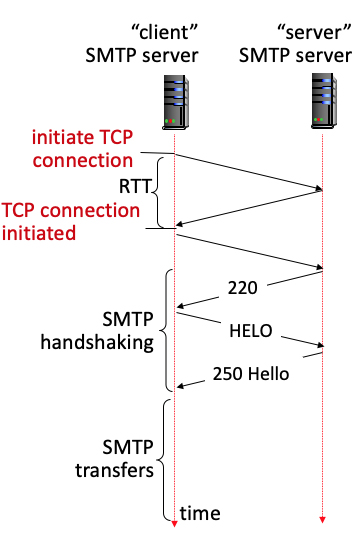
\includegraphics[width=.4\linewidth]{figs/2.3.1.jpg}
\end{center}
\item* 3
\item 0
\item 1
\item 2
\item 2.5
\end{multi}

\begin{multi}[points=1,shuffle,multiple]{2.3-2 Comparing and contrasting HTTP and SMTP.}
\textbf{2.3-2 Comparing and contrasting HTTP and SMTP.} 
Which of the following characteristics apply to HTTP only (and do \emph{not} apply to SMTP)?  
Note: check one or more of the characteristics below.

\item Has ASCII command/response interaction, status codes.
\item Operates mostly as a ``client push'' protocol.
\item[fraction=33.33333] Operates mostly as a ``client pull'' protocol.
\item Is able to use a persistent TCP connection to transfer multiple objects.
\item Uses CRLF.CRLF to indicate end of message.
\item[fraction=33.33333] Uses a blank line (CRLF) to indicate end of request header.
\item[fraction=33.33333] Uses server port 80.
\item Uses server port 25.
\end{multi}

\begin{multi}[points=1,shuffle,multiple]{2.3-3 Comparing and contrasting HTTP and SMTP (2).}
\textbf{2.3-3 Comparing and contrasting HTTP and SMTP (2).} 

Which of the following characteristics apply to SMTP only (and do \emph{not} apply to HTTP)?  
Note: check one or more of the characteristics below.
\item Has ASCII command/response interaction, status codes.
\item[fraction=33.33333] Operates mostly as a ``client push'' protocol.
\item Operates mostly as a ``client pull'' protocol.
\item Is able to use a persistent TCP connection to transfer multiple objects.
\item[fraction=33.33333] Uses CRLF.CRLF to indicate end of message.
\item Uses a blank line (CRLF) to indicate end of request header.
\item Uses server port 80.
\item[fraction=33.33333] Uses server port 25.
\end{multi}

\begin{multi}[points=1,shuffle,multiple]{2.3-4 Comparing and contrasting HTTP and SMTP (3).}
\textbf{2.3-4 Comparing and contrasting HTTP and SMTP (3).} 
Which of the following characteristics apply to both HTTP and SMTP? 
Note: check one or more of the characteristics below.
\item[fraction=50] Has ASCII command/response interaction, status codes.
\item Operates mostly as a ``client push'' protocol.
\item Operates mostly as a ``client pull'' protocol.
\item[fraction=50] Is able to use a persistent TCP connection to transfer multiple objects.
\item Uses CRLF.CRLF to indicate end of message.
\item Uses a blank line (CRLF) to indicate end of request header.
\end{multi}

\begin{matching}[points=1,shuffle]{2.3-5 Which e-mail protocol?}
\textbf{2.3-5 Which e-mail protocol?}  
Match the functionality of a protocol with the name of the email protocol (if any) that implements that functionality.
\item Pushes email from a mail client to a mail server. \answer SMTP
\item Pulls mail from one mail server to another mail server. \answer Neither SMTP nor IMAP does this.
\item Pulls email to a mail client from a mail server. \answer IMAP
\end{matching}

\begin{matching}[points=1,shuffle]{2.4-01 DNS functions.}
\textbf{2.4-01 DNS functions.} 
Match the function of a server to a given type of DNS server in the  DNS server hierarchy.
\item Provides authoritative hostname to IP mappings for organization's named hosts. \answer Authoritative DNS server
\item Replies to DNS query by local host, by contacting other DNS servers to answer the query. \answer Local DNS server
\item Responsible for a domain (e.g., *.com, *.edu); knows how to contact authoritative name servers. \answer Top Level Domain (TLD) servers
\item Highest level of the DNS hierarchy, knows how to reach servers responsible for a given domain (e.g., *.com, *.edu). \answer DNS root servers
\end{matching}

\begin{multi}[points=1,shuffle,multiple]{2.4-02 Why does the local DNS server perform caching?}
\textbf{2.4-02 Why does the local DNS server perform caching?} 
What is the value of caching in the local DNS name server? Check all that apply.

\item[fraction=50] DNS caching provides for faster replies, if the reply to the query is found in the cache.
\item[fraction=50] DNS caching results in less load elsewhere in DNS, when the reply to a query is found in the local cache.
\item DNS caching provides prioritized access to the root servers, since the DNS request is from a local DNS cache.
\item DNS caching provides the ability to serve as authoritative name server for multiple organizations.
\end{multi}

\begin{multi}[points=1,shuffle,multiple]{2.4-03 What's in the DNS type A resource record?}
\textbf{2.4-03 What's in the DNS type A resource record?} 
What information does the type ``A'' resource record hold in the DNS database? Check all that apply.
\item* A hostname and an IP address.
\item A domain name and the name of the authoritative name server for that domain.
\item An alias name and a true name for a server.
\item A name and the name of the SMTP server associated with that name.
\end{multi}

\begin{multi}[points=1,shuffle,multiple]{2.4-04. The local DNS server.}
\textbf{2.4-04. The local DNS server.} 
Check all the phrases below that state a \emph{true} property of a \emph{local} DNS server.
\item[fraction=50] The local DNS server record for a remote host is sometimes different from that of the authoritative server for that host.
\item The local DNS server is only contacted by a local host if that local host is unable to resolve a name via iterative or recursive queries into the DNS hierarchy.
\item The local DNS server holds hostname-to-IP translation records, but not other DNS records such as MX records.
\item[fraction=50] The local DNS server can decrease the name-to-IP-address resolution time experienced by a querying local host over the case when a DNS is resolved via querying into the DNS hierarchy.
\end{multi}

\begin{multi}[points=1,shuffle,multiple]{2.4-05. The DNS authoritative name server.}
\textbf{2.4-05. The DNS authoritative name server.} 
What is the role of an authoritative name server in the DNS? (Check all that apply.)
\item It is a local (to the querying host) server that caches name-to-IP address translation pairs, so it can answer authoritatively and can do so quickly.
\item* It provides the definitive answer to the query with respect to a name in the authoritative name server's domain.
\item It provides the IP address of the DNS server that can provide the definitive answer to the query.
\item It provides a list of TLD servers that can be queried to find the IP address of the DNS server that can provide the definitive answer to this query.
\end{multi}

\begin{multi}[points=1,shuffle]{2.4-06. DNS local caches.}
\textbf{2.4-06. DNS local caches.} 
We saw that a local DNS cache will respond immediately to a client when the local DNS has the name-to-address translation in its local cache. There are millions of such local DNS caches across the Internet. For a given Internet name, will the name-to-address translation pair stored in these local caches always be the same (i.e., are the contents of the local caches synchronized)?

\item* \textbf{No.} The caches are not always synchronized. An entry in a local cache will eventually time out, and the local cache will again eventually go to the DNS hierarchy to get the name-to-address translation pair for this name.  So if the name-to-address mapping changes in the DNS hierarchy, the new mapping will eventually (but not immediately) make its way into the local cache. Therefore, not all local caches may have the same value for name-to-address translation pair.
\item \textbf{No.} The caches are not always synchronized. When a name-to-address mapping changes in the DNS hierarchy, the DNS hierarchy will \emph{push} the new mapping to all local caches.  However,  it takes different amounts of time for these updates to propagate to all local caches. Thus, local caches are not always perfectly synchronized.
\item \textbf{Yes.} The caches are always synchronized.  When a name-to-address mapping changes in the DNS hierarchy, the DNS hierarchy will push to new mapping to all local caches, and the local caches will not install the new mapping until all local caches commit the changes.
\end{multi}

\begin{multi}[points=1,shuffle,multiple]{2.4-07. DNS and HTTP Caching.}
\textbf{2.4-07. DNS and HTTP Caching.} 
We learned that in HTTP web browser caching, HTTP local web server caching, and in local DNS caching, that a user benefits (e.g., shorter delays over the case of no caching) from finding a local/nearby copy of a requested item. 

In which of the following forms of caching does a user benefit not only from its own recent requests and cached replies \emph{but also from recent requests made from other users}?
\item[fraction=50] Local DNS server caching
\item HTTP browser caching
\item[fraction=50] HTTP local web caching
\end{multi}

\begin{multi}[points=1,shuffle]{2.6-1 CDNs.}
\textbf{2.6-1 CDNs.} 
What approach is taken by a CDN to stream content to hundreds of thousands of simultaneous users?
\item Serve video from a single central ``mega-server'' with ultra-high-speed network connectivity, and high-speed storage.
\item* Store/serve multiple copies of videos at multiple geographically distributed sites.
\item Proactively push videos to a client device before they are requested, using machine learning to predict requested videos.
\item Allow client devices to send requested content to each other, in order to offload the CDN infrastructure.
\end{multi}

\begin{matching}[points=1,shuffle]{2.6-2 Streaming video definitions.}
\textbf{2.6-2 Streaming video definitions.} 
Match the definition/function of an element or approach in a networked streaming video system, with its name.
\item A unit of video, each of which may be encoded at multiple different rates, stored in different files. \answer Chunk
\item A file containing the location and encoding rate of files corresponding to video segments in a video. \answer Manifest
\item An approach that allows a client to adapt the encoding rate of retrieved video to network congestion conditions. \answer DASH
\item A CDN approach that stores content in access networks, close to clients. \answer ``Enter deep''
\item \answer Over The Top (OTT)
\item \answer Video frame
\end{matching}

\begin{multi}[points=1,shuffle]{2.6-3 What is DASH?}
\textbf{2.6-3 What is DASH?} 
In DASH (Dynamic, Adaptive Streaming over HTTP), a server divides a video file into chunks that ... (pick best completion from below)
\item* ... are stored, each encoded at multiple rates (video quality). The client plays the video chunk-by-chunk, with each chunk requested at encoding rate that fits the available bandwidth at the time.
\item ... are download smallest-chunk-first in order to maximize the number of chunks received.
\item ... are stored, each encoded at multiple rates (video quality). The client receives multiple video chunks (encoded at different rates) and plays out the chunks that best fit the screen size.
\item ... are downloaded just before their playout time. Chunking is used primarily because a viewer may jump around (e.g., fast forward) in a video.
\item ... allow premium users to avoid watching chunks that contain commercials.
\end{multi}

\begin{multi}[points=1,shuffle]{2.6-4 Manifest file.}
\textbf{2.6-4 Manifest file.} 
What is the purpose of a \emph{manifest file} in a streaming multimedia setting?
\item Allows a video service to log the video and the server from which a client streams a video.
\item To allow a client to reserve bandwidth along a path from a server to that client, so the client can view a stream video without impairment.
\item* To let a client know where it can retrieve different video segments, encoded at different rates
\item To let an OTT (Over-the-top) video server know the video that the client wants to view.
\end{multi}

\begin{multi}[points=1,shuffle,multiple]{2.6-5. Netflix Streaming.}
\textbf{2.6-5. Netflix Streaming.}  
Which of the following (one or more) statements are true about Netflix streaming (check all that are true) or video streaming services in general.
\item Once a video starts streaming from a Netflix server to a client player, the video quality remains constant throughout video playback.
\item Once a video starts streaming from a given Netflix server to a given client player, that server will be the only server assigned to transmit that video to that client throughout the viewing session for this video.
\item* In Netflix, the client requests chunks of video, and each chunk may have a different encoding rate (video quality) and can be retrieved from a different server.
\end{multi}

\begin{multi}[points=1,shuffle,multiple]{2.7-1 UDP Sockets.}
\textbf{2.7-1 UDP Sockets.} 
Which of the following characteristics below are associated with a UDP socket? Check one or more that apply. 
\item \emph{socket(AF\_INET, SOCK\_STREAM)} creates this type of socket
\item[fraction=25] \emph{socket(AF\_INET, SOCK\_DGRAM)} creates this type of socket
\item a server can perform an \emph{accept()} on this type of socket
\item[fraction=25] provides unreliable transfer of a groups of bytes (``a datagram''), from client to server
\item provides reliable, in-order byte-stream transfer (a ``pipe''), from client to server
\item[fraction=25] the application must explicitly specify the IP destination address and port number for each group of bytes written into a socket
\item when contacted, the server will create a new server-side socket to communicate with that client
\item[fraction=25] data from different clients can be received on the same socket
\end{multi}

\begin{multi}[points=1,shuffle,multiple]{2.7-2 TCP Sockets.}
\textbf{2.7-2 TCP Sockets.} 
Which of the following characteristics below are associated with a TCP socket? Check one or more that apply. 
\item[fraction=25] \emph{socket(AF\_INET, SOCK\_STREAM)} creates this type of socket
\item \emph{socket(AF\_INET, SOCK\_DGRAM)} creates this type of socket
\item[fraction=25] a server can perform an \emph{accept()} on this type of socket
\item provides unreliable transfer of a group of bytes (a ``datagram''), from client to server
\item[fraction=25] provides reliable, in-order byte-stream transfer (a ``pipe''), from client to server
\item the application must explicitly specify the IP destination address and port number for each group of bytes written into a socket
\item[fraction=25] when contacted, the server will create a new server-side socket to communicate with that client
\item data from different clients can be received on the same socket
\end{multi}

\begin{multi}[points=1,shuffle]{2.7-3 Server reply (UDP).}
\textbf{2.7-3 Server reply (UDP).} 
How does the networked application running on a server know the client IP address and the port number to reply to in response to a received datagram?
\item* The  application code at the server determines client IP address and port number from the initial segment sent by client, and must explicitly specify these values when sending into a socket back to that client.
\item As the result of performing the \emph{accept()} statement, the server has created a new socket that is bound to that specific client, and so sending into this new socket (without explicitly specifying the client IP address and port number) is sufficient to ensure that the sent data will be addressed to the correct client.
\item The server will query the DNS to learn the IP address of the client.
\item The server will know the port number being used by the client since all services have a well-known port number.
\end{multi}

\begin{multi}[points=1,shuffle]{2.7-4 How many sockets?}
\textbf{2.7-4 How many sockets?} 
Suppose a Web server has \emph{five} ongoing connections that use TCP receiver port 80, and assume there are no other TCP connections (open or being opened or closed) at that server.  How many TCP sockets are in use at this server?
\item* 6
\item 1
\item 4
\item 5
\end{multi}

\begin{multi}[points=1,shuffle]{2.7-5 socket \emph{connect()}.}
\textbf{2.7-5 socket connect().} 
What happens when a socket \emph{connect()} procedure is called/invoked?
\item* This procedure creates a new socket at the client, and connects that socket to the specified server.
\item This causes the client to reach out to a TCP server to establish a connection between that client and the server. If there is already one or more servers on this connection, this new server will also be added to this connection.
\item This causes the server to reach out to a TCP client to establish a connection between that client and the server.
\end{multi}

\end{quiz}
\end{document}
